%%%%%%%%%%%%%%%%%%%%%%%%%%%%%%%%%%%%%%%%%%%%%%%%%%%%%%%%%%%%%%%%%%%%%%%%%%%%%%%%
% file:   basicsLaTeX.Rnw
% author: Peter DeWitt, peter.dewitt@ucdenver.edu
% 
% For:    Example Rnw file for creating a data analysis report using R, knitr,
% and LaTeX.
%
% Please read the introduction section in this file, or the resulting pdf, for
% instructions on reproducing the data analysis report.  
%
% change log:
% 11 Nov 2013 - File created
%
%%%%%%%%%%%%%%%%%%%%%%%%%%%%%%%%%%%%%%%%%%%%%%%%%%%%%%%%%%%%%%%%%%%%%%%%%%%%%%%%

% Preamble %{{{ 
\documentclass[letterpaper, 10pt]{article}\usepackage[]{graphicx}\usepackage[]{color}
%% maxwidth is the original width if it is less than linewidth
%% otherwise use linewidth (to make sure the graphics do not exceed the margin)
\makeatletter
\def\maxwidth{ %
  \ifdim\Gin@nat@width>\linewidth
    \linewidth
  \else
    \Gin@nat@width
  \fi
}
\makeatother

\definecolor{fgcolor}{rgb}{0.345, 0.345, 0.345}
\newcommand{\hlnum}[1]{\textcolor[rgb]{0.686,0.059,0.569}{#1}}%
\newcommand{\hlstr}[1]{\textcolor[rgb]{0.192,0.494,0.8}{#1}}%
\newcommand{\hlcom}[1]{\textcolor[rgb]{0.678,0.584,0.686}{\textit{#1}}}%
\newcommand{\hlopt}[1]{\textcolor[rgb]{0,0,0}{#1}}%
\newcommand{\hlstd}[1]{\textcolor[rgb]{0.345,0.345,0.345}{#1}}%
\newcommand{\hlkwa}[1]{\textcolor[rgb]{0.161,0.373,0.58}{\textbf{#1}}}%
\newcommand{\hlkwb}[1]{\textcolor[rgb]{0.69,0.353,0.396}{#1}}%
\newcommand{\hlkwc}[1]{\textcolor[rgb]{0.333,0.667,0.333}{#1}}%
\newcommand{\hlkwd}[1]{\textcolor[rgb]{0.737,0.353,0.396}{\textbf{#1}}}%

\usepackage{framed}
\makeatletter
\newenvironment{kframe}{%
 \def\at@end@of@kframe{}%
 \ifinner\ifhmode%
  \def\at@end@of@kframe{\end{minipage}}%
  \begin{minipage}{\columnwidth}%
 \fi\fi%
 \def\FrameCommand##1{\hskip\@totalleftmargin \hskip-\fboxsep
 \colorbox{shadecolor}{##1}\hskip-\fboxsep
     % There is no \\@totalrightmargin, so:
     \hskip-\linewidth \hskip-\@totalleftmargin \hskip\columnwidth}%
 \MakeFramed {\advance\hsize-\width
   \@totalleftmargin\z@ \linewidth\hsize
   \@setminipage}}%
 {\par\unskip\endMakeFramed%
 \at@end@of@kframe}
\makeatother

\definecolor{shadecolor}{rgb}{.97, .97, .97}
\definecolor{messagecolor}{rgb}{0, 0, 0}
\definecolor{warningcolor}{rgb}{1, 0, 1}
\definecolor{errorcolor}{rgb}{1, 0, 0}
\newenvironment{knitrout}{}{} % an empty environment to be redefined in TeX

\usepackage{alltt}
\usepackage{fullpage}
\usepackage{url}
\usepackage{verbatim}
\usepackage{ctable}

\title{Example Data Analysis Report\\Reproducible Research Using {\tt knitr}
with \LaTeX}
\author{Peter DeWitt}




% End Preamble %}}}

%%%%%%%%%%%%%%%%%%%%%%%%%%%%%%%%%%%%%%%%%%%%%%%%%%%%%%%%%%%%%%%%%%%%%%%%%%%%%%%%
\IfFileExists{upquote.sty}{\usepackage{upquote}}{}
\begin{document}

\maketitle

\section{Introduction \label{sec:introduction}}  %{{{

This document serves as an example data analysis report generated using R for
the analysis, \LaTeX\ for the markup report writing language, and knitr to bring
everything together.   The data set used is a fictitious as was generated for
example purposes only.  The purpose of this document is to provide an example of
reproducible research.

\paragraph{Reproducing this report}  These are the steps required for
reproducing this report.
\begin{enumerate}
  \item Install R and \LaTeX\ on your computer.

  \item Open R, install the knitr package if the package is not on your system.
% This chunk is for example purposes only, not be evaluated
\begin{knitrout}
\definecolor{shadecolor}{rgb}{0.969, 0.969, 0.969}\color{fgcolor}\begin{kframe}
\begin{alltt}
\hlkwd{install.packages}\hlstd{(}\hlstr{"knitr"}\hlstd{,} \hlkwc{repos} \hlstd{=} \hlstr{"http://cran.rstudio.com"}\hlstd{)}
\end{alltt}
\end{kframe}
\end{knitrout}


  \item Set the working directory in R to the same directory as this file exists
    in.  Run the following commands in R, 
% This chunk is for example purposes only, not be evaluated
\begin{knitrout}
\definecolor{shadecolor}{rgb}{0.969, 0.969, 0.969}\color{fgcolor}\begin{kframe}
\begin{alltt}
\hlkwd{library}\hlstd{(knitr)}
\hlkwd{knit}\hlstd{(}\hlkwc{input} \hlstd{=} \hlstr{"basicsLaTeX.Rnw"}\hlstd{)}
\end{alltt}
\end{kframe}
\end{knitrout}


  \item The above R code will generate the file {\tt basicLaTeX.tex}.  Use your
    favorite \LaTeX\ compiler to generate the .pdf, .eps, .ps, \ldots.  If you
    get a copy of the directory with the auxiliary files resulting from compiling
    the \LaTeX, such as .aux, .log, \ldots, please delete those files.  Only the
    .Rnw file is truly necessary to reproduce this report.
\end{enumerate}

% end sec:introduction %}}}

\section{Analysis Methods \label{sec:methods}} %{{{

Overall survival analysis was done using both
Kaplan-Meier estimates and Cox proportional hazard regression models.  
The analysis was done in R version 3.0.2 (2013-09-25)~\cite{R-base} and the
survival analysis was done using the {\tt survival} package~\cite{R-survival}.
Statistical significance was set at the 0.05 level.

% end sec:methods %}}}

\section{Analysis and Results \label{sec:analysis}} %{{{




The data set consisted of 19,039
records.  A summary of the data set is presented
in Table~\ref{tab:demographics}.  

% latex.default(tab, file = "", title = "", ctable = TRUE, caption = "Data Set summary",      label = "tab:demographics", cgroup = c("Overall", paste("GS",          7:10)), n.cgroup = rep(2, 5), colhead = rep(c("n", "\\%"),          5), extracolheads = clhd, rgroup = c("Age (in years)",          "Era", "PSA", "T Stage", "Observed Deaths"), n.rgroup = c(3,          2, 3, 3, 1), col.just = rep("r", ncol(tab))) 
%
\ctable[caption={Data Set summary},label=tab:demographics,pos=!tbp,]{lrrcrrcrrcrrcrr}{}{\FL
\multicolumn{1}{l}{\bfseries }&\multicolumn{2}{c}{\bfseries Overall}&\multicolumn{1}{c}{\bfseries }&\multicolumn{2}{c}{\bfseries GS 7}&\multicolumn{1}{c}{\bfseries }&\multicolumn{2}{c}{\bfseries GS 8}&\multicolumn{1}{c}{\bfseries }&\multicolumn{2}{c}{\bfseries GS 9}&\multicolumn{1}{c}{\bfseries }&\multicolumn{2}{c}{\bfseries GS 10}\NN
\cline{2-3} \cline{5-6} \cline{8-9} \cline{11-12} \cline{14-15}
\multicolumn{1}{l}{}&\multicolumn{1}{c}{n}&\multicolumn{1}{c}{\%}&\multicolumn{1}{c}{}&\multicolumn{1}{c}{n}&\multicolumn{1}{c}{\%}&\multicolumn{1}{c}{}&\multicolumn{1}{c}{n}&\multicolumn{1}{c}{\%}&\multicolumn{1}{c}{}&\multicolumn{1}{c}{n}&\multicolumn{1}{c}{\%}&\multicolumn{1}{c}{}&\multicolumn{1}{c}{n}&\multicolumn{1}{c}{\%}\NN
&\multicolumn{1}{c}{{\scriptsize 19,039}}&&&\multicolumn{1}{c}{{\scriptsize 12,986}}&\multicolumn{1}{c}{{\scriptsize 68.21}}&&\multicolumn{1}{c}{{\scriptsize 3,670}}&\multicolumn{1}{c}{{\scriptsize 19.28}}&&\multicolumn{1}{c}{{\scriptsize 2,139}}&\multicolumn{1}{c}{{\scriptsize 11.23}}&&\multicolumn{1}{c}{{\scriptsize 244}}&\multicolumn{1}{c}{{\scriptsize 1.28}}\ML
{\bfseries Age (in years)}&&&&&&&&&&&&&&\NN
~~[40,50)&3,051&16.03&&2,145&16.52&&544&14.82&&323&15.10&&39&15.98\NN
~~[50,70)&5,945&31.23&&4,259&32.80&&1,005&27.38&&608&28.42&&73&29.92\NN
~~[70,85]&10,043&52.75&&6,582&50.69&&2,121&57.79&&1,208&56.47&&132&54.10\ML
{\bfseries Era}&&&&&&&&&&&&&&\NN
~~Era 1&8,615&45.25&&5,869&45.19&&1,659&45.20&&970&45.35&&117&47.95\NN
~~Era 2&10,424&54.75&&7,117&54.81&&2,011&54.80&&1,169&54.65&&127&52.05\ML
{\bfseries PSA}&&&&&&&&&&&&&&\NN
~~[0, 10) ng/ml&11,567&60.75&&8,410&64.76&&1,997&54.41&&1,038&48.53&&122&50.00\NN
~~[10, 20) ng/ml&4,372&22.96&&2,845&21.91&&927&25.26&&531&24.82&&69&28.28\NN
~~[20, Inf) ng/ml&3,100&16.28&&1,731&13.33&&746&20.33&&570&26.65&&53&21.72\ML
{\bfseries T Stage}&&&&&&&&&&&&&&\NN
~~T Stage 1&9,668&50.78&&7,110&54.75&&1,699&46.29&&770&36.00&&89&36.48\NN
~~T Stage 2&8,189&43.01&&5,360&41.28&&1,657&45.15&&1,065&49.79&&107&43.85\NN
~~T Stage 3/4&1,182&6.21&&516&3.97&&314&8.56&&304&14.21&&48&19.67\ML
{\bfseries Observed Deaths}&&&&&&&&&&&&&&\NN
~~&2,755&&&1,611&&&598&&&473&&&73&\LL
}




\begin{knitrout}
\definecolor{shadecolor}{rgb}{0.969, 0.969, 0.969}\color{fgcolor}\begin{figure}[]


{\centering 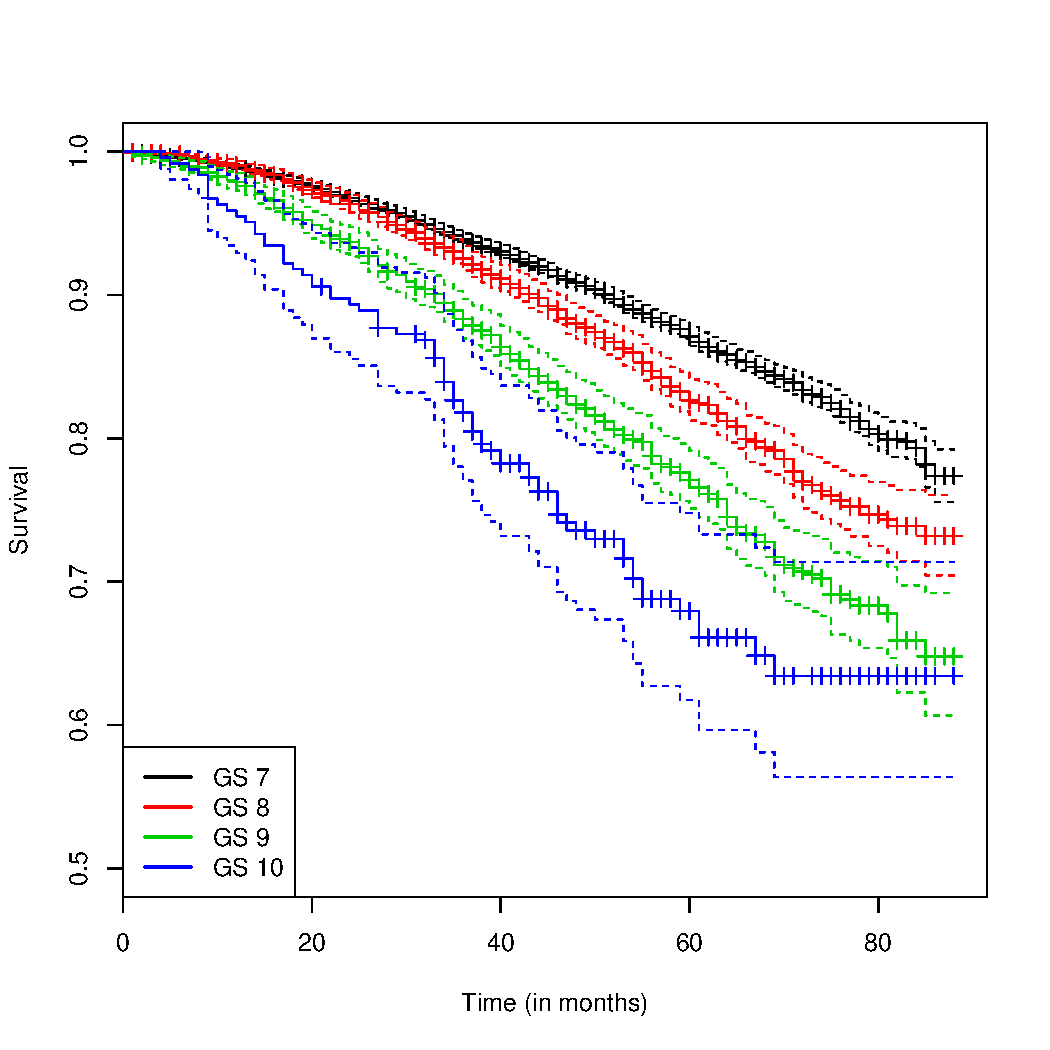
\includegraphics[width=0.48\textwidth]{figure/km_plot} 

}

\caption[Kaplam-Meier Survival Curves]{Kaplam-Meier Survival Curves\label{fig:km_plot}}
\end{figure}


\end{knitrout}


We are primarily interested in the differences in survival between patients with
different Gleason scores.  Figure~\ref{fig:km_plot} presents the Kaplan-Meier
survival estimates by Gleason score.  As expected, the higher the Gleason score,
the worse the survival.  It should also be noted that even after seven years of
tracking patients the median survival time is not estimable.  The lowest
survival estimate is 63.43\%.

Both univariable and multivariable Cox proportional hazard regression models
were fitted for overall survival by the age, era of treatment, T stage, PSA, and
Gleason score of the patient.  Results for all the regression models are
presented in Table~\ref{tab:coxph}.  

% latex.default(coxph.results, file = "", title = "", ctable = TRUE,      caption = cap, label = "tab:coxph", cgroup = c("Univariable Regressions",          "Multivariable Regression"), n.crgoup = rep(4, 2), colhead = rep(c("HR",          "LCL", "UCL", "p-value"), 2), rgroup = rgrp, n.rgroup = nrgrp,      rowname = rwnm, col.just = rep("r", ncol(coxph.results))) 
%
\ctable[caption={Hazard ratios (HR) along with 95\% confidence intervals (LCL, UCL) and
p-values for testing if the hazard ratio is statistically different from 1 are
presented in this table for both univariable and multivariable regression models
for overall survival.},label=tab:coxph,pos=!tbp,]{lrrrrcrrrr}{}{\FL
\multicolumn{1}{l}{\bfseries }&\multicolumn{4}{c}{\bfseries Univariable Regressions}&\multicolumn{1}{c}{\bfseries }&\multicolumn{4}{c}{\bfseries Multivariable Regression}\NN
\cline{2-5} \cline{7-10}
\multicolumn{1}{l}{}&\multicolumn{1}{c}{HR}&\multicolumn{1}{c}{LCL}&\multicolumn{1}{c}{UCL}&\multicolumn{1}{c}{p-value}&\multicolumn{1}{c}{}&\multicolumn{1}{c}{HR}&\multicolumn{1}{c}{LCL}&\multicolumn{1}{c}{UCL}&\multicolumn{1}{c}{p-value}\ML
{\bfseries Age}&&&&&&&&&\NN
~~[40,50)&Reference&&&&&Reference&&&\NN
~~[50,70)&0.95&0.84&1.09&0.4807&&0.96&0.84&1.10&0.5550\NN
~~[70,85]&1.62&1.44&1.81&\textless 0.0001&&1.61&1.43&1.80&\textless 0.0001\ML
{\bfseries Era}&&&&&&&&&\NN
~~Era 1&Reference&&&&&Reference&&&\NN
~~Era 2&0.83&0.76&0.90&\textless 0.0001&&0.84&0.77&0.92&\textless 0.0001\ML
{\bfseries T.Stage}&&&&&&&&&\NN
~~T Stage 1&Reference&&&&&Reference&&&\NN
~~T Stage 2&1.19&1.10&1.29&\textless 0.0001&&1.12&1.03&1.21&0.0063\NN
~~T Stage 3/4&1.54&1.34&1.77&\textless 0.0001&&1.24&1.07&1.43&0.0033\ML
{\bfseries PSA}&&&&&&&&&\NN
~~[0, 10) ng/ml&Reference&&&&&Reference&&&\NN
~~[10, 20) ng/ml&1.45&1.32&1.58&\textless 0.0001&&1.36&1.24&1.48&\textless 0.0001\NN
~~[20, Inf) ng/ml&1.62&1.47&1.78&\textless 0.0001&&1.50&1.36&1.66&\textless 0.0001\ML
{\bfseries Gleason}&&&&&&&&&\NN
~~GS 7&Reference&&&&&Reference&&&\NN
~~GS 8&1.34&1.22&1.47&\textless 0.0001&&1.23&1.12&1.35&\textless 0.0001\NN
~~GS 9&1.92&1.73&2.12&\textless 0.0001&&1.73&1.55&1.91&\textless 0.0001\NN
~~GS 10&2.74&2.17&3.46&\textless 0.0001&&2.48&1.96&3.14&\textless 0.0001\LL
}






The results of a univariable regression model indicated that 
Patients treated in Era 2 had statistically better survival than patients
treated in Era 1, HR = 0.83 (95\% CI: 0.76,0.90), and there was no
appreciable difference in the hazard ratio found in the multivariable
regression model, HR = 0.84 (95\% CI: 0.77,0.92).  As expected, as
patients increase in age, T Stage increase, PSA increase, and Gleason score
increases, the hazard also increases.

The hazard ratio between Gleason 8 and Gleason 7, from the multivariable Cox
proportional hazard regression model, is 
HR = 1.23 (95\% CI: 1.12,1.35).  
Further analysis of the pairwise comparisons of the hazards between all
four Gleason scores can be provided upon request.

% End sec:analysis %}}}

\section{Conclusions \label{sec:conclusions}} %{{{
The conclusions section for a data analysis report would generally be used to
summarize the results presented in Section~\ref{sec:analysis}, list any
limitations to the study, and generate some discussion topics.  Seeing how the
purpose of {\it this} report was to show illustrate the use of {\tt knitr}, the
conclusions will focus on reproducible research.

Using {\tt knitr} to write data analysis reports were the written report and the
data analysis methods is a version of literate programming.  When written well,
the report are robust to changes in the data set, but more importantly, every
element of the report is commented directly or contextually.  

In addition to using {\tt knitr}, a very powerful tool for authoring reports,
both as a sole author, or as a collaboration, is to use version control
software.  I prefer {\tt git}\footnote{\url{http://git-scm.com/}}, but another
viable option is subversion.  RStudio has built-in features to working with
either.  Repository hosting on github.com or bitbucket.org are helpful, but on
public servers (private repos are possible, but think about the physical
location of the data storage).  The git server software can be purchased and set
up behind institutional firewalls.  

% end sec:conclusions %}}}

% Backmatter %{{{




\bibliographystyle{apalike}
\bibliography{R-sources}

\appendix

\begin{knitrout}
\definecolor{shadecolor}{rgb}{0.969, 0.969, 0.969}\color{fgcolor}\begin{kframe}
\begin{alltt}
\hlcom{# for reproducability, print out the session infor for the packages, and}
\hlcom{# versions of the packages, used to run the anlaysis and create this}
\hlcom{# document.}
\hlkwd{print}\hlstd{(}\hlkwd{sessionInfo}\hlstd{(),} \hlkwc{local} \hlstd{=} \hlnum{FALSE}\hlstd{)}
\end{alltt}
\begin{verbatim}
## R version 3.0.2 (2013-09-25)
## Platform: x86_64-pc-linux-gnu (64-bit)
## 
## attached base packages:
## [1] splines   stats     graphics  grDevices utils     datasets  methods  
## [8] base     
## 
## other attached packages:
## [1] gdata_2.13.2    Hmisc_3.12-2    Formula_1.1-1   survival_2.37-4
## [5] knitr_1.4.1     vimcom_0.9-9    setwidth_1.0-3  colorout_1.0-0 
## 
## loaded via a namespace (and not attached):
##  [1] cluster_1.14.4  digest_0.6.3    evaluate_0.4.7  formatR_0.9    
##  [5] grid_3.0.2      gtools_3.1.0    highr_0.2.1     lattice_0.20-24
##  [9] rpart_4.1-3     stringr_0.6.2   tools_3.0.2
\end{verbatim}
\end{kframe}
\end{knitrout}

% end backmatter %}}}

\end{document}
%%%%%%%%%%%%%%%%%%%%%%%%%%%%%%%%%%%%%%%%%%%%%%%%%%%%%%%%%%%%%%%%%%%%%%%%%%%%%%%%
%%%% END OF FILE %% END OF FILE % END OF FILE %% END OF FILE %% END OF FILE %%%%
%%%%%%%%%%%%%%%%%%%%%%%%%%%%%%%%%%%%%%%%%%%%%%%%%%%%%%%%%%%%%%%%%%%%%%%%%%%%%%%%

